\chapter{Célértékkeresés}
\thispagestyle{empty}

A Calcban megadhatjuk, hogy egy képlet vagy függvény általunk
meghatározott eredményt adjon. Természetesen megadva azt a
paramétert (cellát), amelyiket a program módosíthat a
kívánt eredmény eléréséhez. Ezt a módszert célértékkeresésnek nevezzük.

A célértékkeresést gyakran alkalmazzák pénzügyi,
mérnöki és matematikai számításoknál.

Vizsgáljuk meg ismét az FV függvényt bemutató feladatot. 
(\ref{Célértékkeresés} ábra) Határozzuk meg célértékkereséssel,
hogy mekkora összeget kell elhelyeznünk egy 12\% évi kamatozású
számlán,  hogy 20~000~Ft-ot befizetve minden hó végén 5
éven át a számlán kétmillió forint legyen.

\begin{figure}[!h]
\begin{center}
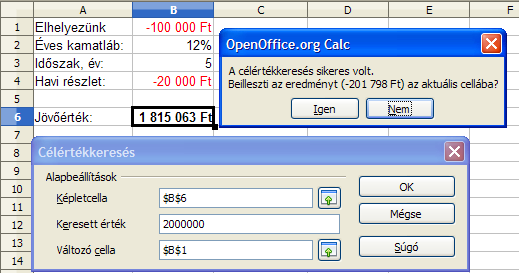
\includegraphics[width=13.73cm]{oocalcv1-img140.png}
\caption{Célértékkeresés}\label{Célértékkeresés}
\end{center}
\end{figure}

Az \textbf{Eszközök} menüpont \textbf{Célértékkeresés}
ablakában a \textbf{Képletcella} a B6 lesz, az a cella amelyikben
egy konkrét eredményt akarunk elérni. A \textbf{Keresett
érték} részbe be kell írnunk ezt az értéket. A
\textbf{Változó cella} a B1, ezt módosítja a Calc. Az Ok gombot
választva a  program megjeleníti a célértékkeresés
eredményét. Az \textbf{Igen} gombbal beilleszthetjük a
megtalált értéket a B1 cellába (\ref{Célértékkeresés} ábra).


\section{32. feladat}

\textit{Találjuk meg célértékkeresés segítségével azt az
értékét az x-nek, amikor }
$\frac{20}{x^{2}+3}=x-\frac{5}{x^{2}+1}$\textit{.  Oldjuk meg
grafikusan is az egyenletet.}

Számítsuk ki a kifejezés bal és jobb oldalát a B1 cellába
írt értéket tekintve $x$-nek. Ellenőrzésképpen
írjunk nullát a B1-be. A két érték különbségét
meghatározva az E5 cellában, célértékkeresés
segítségével meghatározhatjuk a B1 cellában azt a számot,
amelyiknél az E5 értéke nulla lesz (\ref{32-feladatCélérték} ábra).

\begin{figure}[!h]
\begin{center}
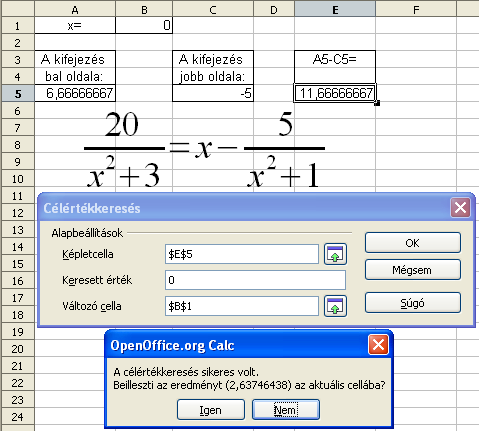
\includegraphics[width=12.674cm]{oocalcv1-img141.png}
\caption{32. feladat --  Célértékkeresés}\label{32-feladatCélérték}
\end{center}
\end{figure}

Az eredmény megközelítőleg 2,637. 

A \textbf{Beszúrás} menüpont \textbf{Objektum} --  \textbf{Képlet}
paranccsal hozhatjuk létre \aref{32-feladatCélérték} ábrán látható
matematikai kifejezést.

Grafikusan úgy ábrázolhatjuk az egyenlet megoldását, hogy a
kifejezés jobb és bal oldalát függvényeknek tekintjük és
közös koordináta rendszerben ábrázoljuk a grafikonjaikat. A
grafikonok  metszéspontjainak x koordinátái adjak a megoldást,
vagy megoldásokat. A y koordináták pedig azt az értéket, amit
ilyenkor a két függvény felvesz.

Számítsuk ki a kifejezés bal és jobb oldalát a [-10;10]
intervallumon 0,1 lépéssel, és építsünk Pont(XY) diagramot
(sima vonalak altípus, csak vonalak bekapcsolva) az A1:C202
tartomány adataiból. Az \textbf{Adatsor} tulajdonságainál, az
\textbf{Ikon} résznél válasszunk a \textbf{Nincs szimbólum}
beállítást (\ref{32-feladatGrafikon} ábra).

\begin{figure}[!h]
\begin{center}
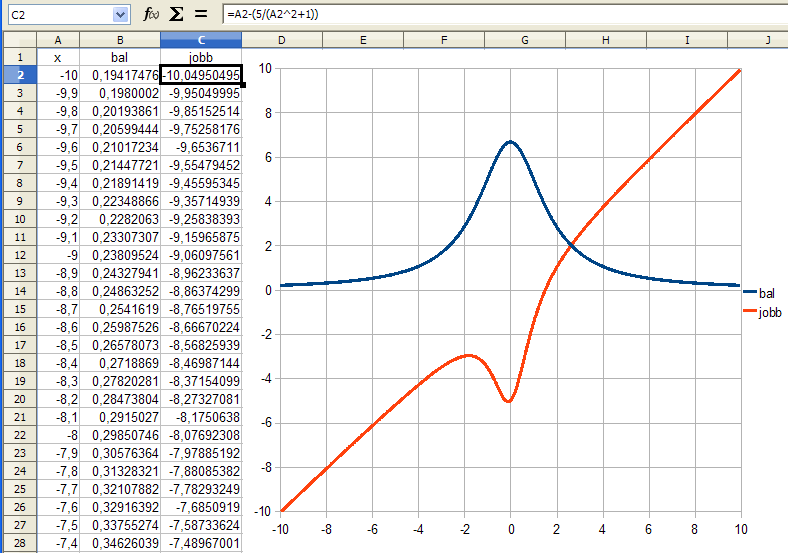
\includegraphics[width=15.999cm]{oocalcv1-img142.png}
\caption{32. feladat -- grafikon}\label{32-feladatGrafikon}
\end{center}
\end{figure}

Módosítsuk a diagram X és Y tengelyének
skálabeállításait, hogy nagyobb pontossággal
megbecsülhessük a grafikonok metszéspontjának koordinátáit.
Az X tengely beállításait \aref{32-feladatXtengely} ábrán látjuk.

\begin{figure}[!h]
\begin{center}
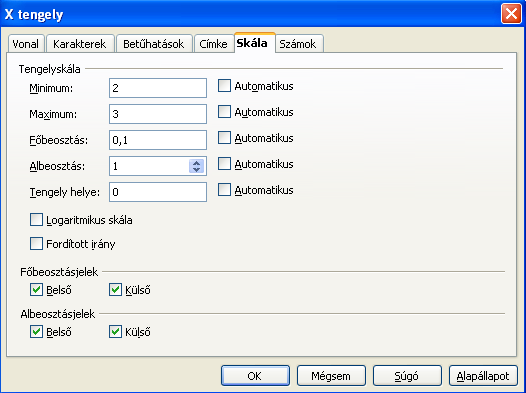
\includegraphics[width=12.917cm]{oocalcv1-img143.png}
\caption{32. feladat --  X tengely}\label{32-feladatXtengely}
\end{center}
\end{figure}

Az Y tengelynél a minimum értéke legyen 1,5 a maximum pedig 2,5. A
többi beállítás megegyezik az X tengelyével. Ezekkel a
tengelybeállításokkal a diagram \aref{32-feladatMegoldás} ábrán látható.
A metszéspont X koordinátája kb. 2,64, ami megegyezik a
célértékkereséssel meghatározott értékkel. \Aref{32-feladatMegoldás}
ábrán látható grafikon alapján biztosra vehetjük, hogy csak
egy megoldása van az egyenletnek.

\begin{figure}[!h]
\begin{center}
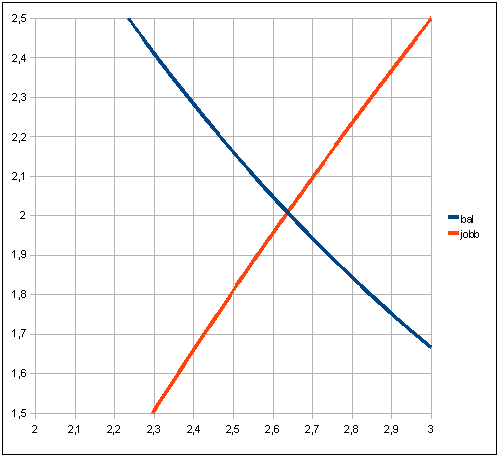
\includegraphics[width=12.203cm]{oocalcv1-img144.png}
\caption{32. feladat -- megoldás}\label{32-feladatMegoldás}
\end{center}
\end{figure}

